\chapter{Espaces préhilbertiens ou euclidiens}
\labch{espaces_prehilbertiens_ou_euclidiens}

Lorsque $E$ est un espace euclidien, le procédé de \textsc{Gram}-\textsc{Schmidt} permet, à partir d'une base adaptée à un drapeau total de $E$, d'obtenir une base orthonormale adaptée à ce même drapeau. \\
Si l'on combine avec le théorème de trigonalisation utilisant les drapeaux, on constate que tout endomorphisme trigonalisable peut être trigonalisé dans une base orthonormale. 

\section{Déterminant de \textsc{Gram}} \label{matrice_gram}
\begin{tcolorbox}
    Soit $E$ un espace euclidien et $(x_1, \dots, x_p)$ une famille d'éléments de $E$. On définit
    $$\text{la matrice de \textsc{Gram} } \Gram = \left( \langle x_i, x_j \rangle \right)_{i,j \in \llbracket 1, p \rrbracket}$$
    $$\text{le déterminant de \textsc{Gram} } \Gram(x_1, \dots, x_p) = \det \Gram.$$
    On remarque que $\Gram$ est symétrique. 
    Le déterminant de \textsc{Gram} permet de calculer des volumes et de tester l'indépendance linéaire d'une famille de vecteurs.
\end{tcolorbox}

Résultats: à compléter à partir de \url{https://fr.wikipedia.org/wiki/Déterminant_de_Gram}
\begin{itemize}
    \item La matrice de \textsc{Gram} est toujours positive.
    \item La famille $(x_1, \dots, x_p)$ et sa matrice de \textsc{Gram} ont le même rang.
    \item La famille $(x_1, \dots, x_p)$ est liée si et seulement si $\det \Gram(x_1, \dots, x_p) = 0$.
    \item Soit $F = \Vect(x_1, \dots, x_p)$,
    $$\forall x \in E,\ \det \Gram(x, x_1, \dots, x_p) = d^2(x, F) \times \det \Gram(x_1, \dots, x_p)$$
\end{itemize} 

\begin{enumerate}
    \item Montrer que la famille $(x_1, \dots, x_p)$ est liée si et seulement si $\Gram(x_1, \dots, x_p) = 0$. \\
    $(\Rightarrow)$ Il existe une famille $(\lambda_1, \dots, \lambda_p)$ non nulle  de $\R^n$ telle que $\sum\limits_{i=1}^{p} \lambda_i x_i = 0$. On montre alors que pour tout ligne $L_i$ de $\Gram$, $\sum\limits_{i=1}^{p} \lambda_i L_i = 0$ ce qui permet de conclure. \\
    $(\Leftarrow)$ Raisonner par contraposée, on suppose $\mathscr{F}$ libre. \\
    Soit $\mathscr{B} = (\varepsilon_1, \dots, \varepsilon_n)$ une b.o.n. de $E$ et $H \in \M_{n, p} (\R)$ la matrice de $\mathscr{F} = (x_1, \dots, x_p)$ dans $\mathscr{B}$. \\
    Alors $\boxed{\Trsp{H} H = G(x_1, \dots, x_p)}$. \\
    Montrons la chaîne :
    $$\Rg(G) = \underbrace{\Rg(\Trsp{H} H) = \Rg(H)}_{\text{à montrer}} = \Rg(\mathscr{F}) = p \not= 0$$
    Montrer que $\Rg(\Trsp{H} H) = \Rg(H)$ en montrant que $\Ker(\Trsp{H} H) = \Ker(H)$. 
    \begin{itemize}
        \item $(\subset)$ oui
        \item $(\supset)$ Soit $X \in \Ker(\Trsp{H}H)$. On montre que $\norme{BX} = 0 \Rightarrow BX = 0$. 
    \end{itemize}
    Par le \textbf{théorème du rang}, on obtient le résultat. 
\end{enumerate}

\begin{tcolorbox}
    La matrice de \textsc{Gram} est symétrique positive.
\end{tcolorbox}

\begin{proof} \\

    \begin{itemize}
        \item La matrice de \textsc{Gram} est symétrique par symétrie du produit scalaire.
        \item Montrons la positivité de $\Gram$. Soit $X = \Trsp{(\alpha_1 \cdots \alpha_n)} \in \M_{n,1}(\R)$. Montrons que $\Trsp{X} \Gram X \geqslant 0$. 
        \begin{align*}
            \Trsp{X} \Gram X &= \sum_{i=1}^{n} \sum_{j=1}^{n} \langle x_i, x_j \rangle \alpha_i \alpha_j \\ 
            &= \sum_{i=1}^{n} \sum_{j=1}^{n} \langle \alpha_i x_i, \alpha_j x_j \rangle \\
            &= \left\Vert \sum_{i=1}^{n}x_i \alpha_i \right\Vert^2 \geqslant 0.
        \end{align*}
    \end{itemize}
   
    Ce qui montre bien que $\Gram$ est symétrique positive.
\end{proof}

\marginnote[-4cm]{
    \begin{kaobox}[frametitle=Matrices symétriques positives]
        L'ensemble des \emph{matrices symétriques positives} est noté $\mathscr{S}_n^+(\R)$. Une matrice $M \in \mathscr{S}_n^+(\R)$ équivaut à chacune des propriétés suivantes:
        \begin{itemize}
            \item pour tout $X \in \M_n(\R), \Trsp{X} M X \geqslant 0$,
            \item $\Sp(M) \subset \Rp.$
        \end{itemize}
    \end{kaobox}
}


\section{Positivité de la matrice de \textsc{Hilbert}}
\marginnote[0cm]{(Planche n°14. Espaces euclidiens de \cite{maths-france})}
Si on interprète le terme général de la matrice de \textsc{Hilbert} (cf. \nameref{matrice_hilbert}) comme 
$$\Hilb_{i,j} = \int_{0}^{1} x^{i+j-2} \d x$$
on peut y reconnaître une \nameref{matrice_gram} pour les fonctions puissances et le produit scalaire usuel sur l'espace des fonctions de $[0, 1]$ dans $\R$ de carré intégrable. Puisque les fonctions puissances sont linéairement indépendantes, les matrices de \textsc{Hilbert} sont donc
\href{https://fr.wikipedia.org/wiki/Matrice_de_Hilbert}{définies positives}.


\section{Inégalité d'\textsc{Hadamard}}
%\begin{marginfigure}[-1cm]
%    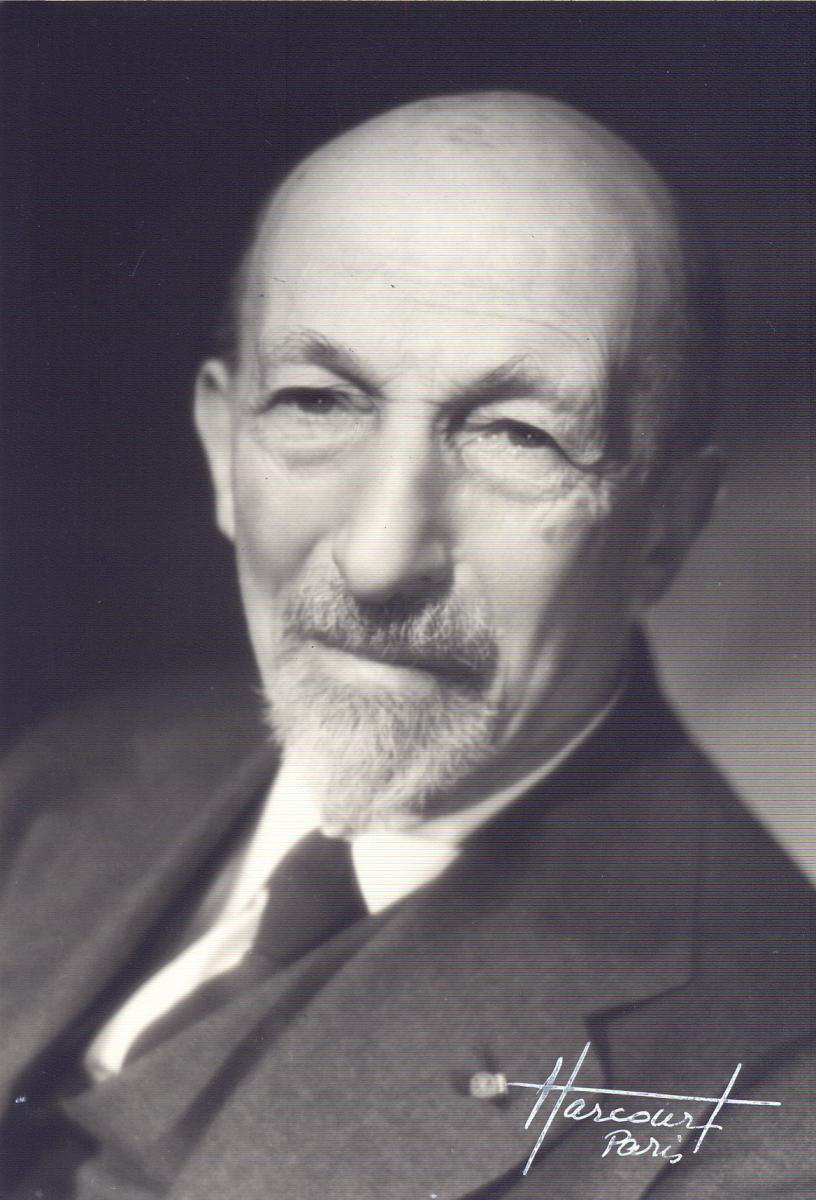
\includegraphics[width=5cm]{images/jacques_hadamard.jpg}
%    \caption{Jacques \textsc{Hadamard}}
%\end{marginfigure}

\begin{theo}{Inégalité d'\textsc{Hadamard}}
    Soit $M \in \M_n(\C)$ et soient $X_1, \dots, X_n$ ses vecteurs colonnes. Alors,
    $$|\mathrm{det} M | \leqslant \prod_{i=1}^{n} \Vert X_i \Vert$$
    avec égalité si et seulement si la famille $(X_i)_{1 \leqslant i \leqslant n}$ est orthogonale.
\end{theo}

%\begin{marginfigure}[-2cm]
%    \resizebox{6.5cm}{6.5cm}{%
    \begin{tikzpicture}
        \node[block] (gram) {Déterminant \\ de \textsc{Gram}};
        \node[block, right of=s1] (iwasama) {Décomposition \\ d'\textsc{Iwasama}};
        \node[block, below right of=gram] (hadamard) {Inégalité \\ d'\textsc{Hadamard}};
    
        \draw (gram) edge[bend right, above left] node {...} (hadamard);
    
        \draw (iwasama) edge[bend left] node {$M=OT$} (hadamard);
    
    \end{tikzpicture}    
}
%\end{marginfigure}

Voyons deux démonstrations de ce résultat; une première en utilisant la décomposition d'\textsc{Iwasama} et une deuxième le \refthm{inegalite_gram}.

\begin{preuve}
    \begin{itemize}
        \item Si la matrice $M$ n'est pas inversible alors $\det M = 0$ et comme une norme est à valeurs positives, le résultat est immédiat. 
        \item Supposons que $M$ est inversible. D'après la décomposition d'\textsc{Iwasama}, il existe une matrice $O \in \mathscr{O}_n(\C)$ et $T \defeq (t_{i,j})_{1 \leqslant i, j \leqslant n}$, triangulaire supérieure dont les coefficients diagonaux sont strictement positifs telles que $M = OT$. D'après la multiplicité du déterminant, 
        $$\det M = \det(O) \det(T).$$
        Or $\det O = \pm 1$ donc
        \begin{equation} \label{det}
            |\det M | = |\det T | = \prod_{i=1}^{n} |t_{i,i}|.
        \end{equation}
        Par construction, pour tout $i \in \llbracket 1, n \rrbracket, t_{i,i} \defeq \langle X_i, O_i \rangle$ où $O_i$ est un vecteur unitaire. D'après l'inégalité de \textsc{Cauchy}-\textsc{Schwarz}, pour tout $i \in \llbracket 1, n \rrbracket$, 
        $$|t_{i,i}| = |\langle X_i, O_i \rangle | \leqslant \norme{X_i} \underbrace{\norme{O_i}}_{=1}.$$
        Ainsi d'après (\ref{det}), 
        $$|\det(M)| \leqslant \prod_{i=1}^n \norme{X_i}.$$
    \end{itemize}
        \textcolor{red}{cas d'égalité}
\end{preuve}

\begin{preuve}
    \begin{itemize}
        \item Si la matrice $M$ n'est pas inversible, le résultat est immédiat. 
        \item Supposons que $M$ est inversible. On a 
        $$\Trsp{M} M = \Gram(X_1, \dots, X_n),$$ 
        la matrice de \textsc{Gram} de la famille des colonnes de la matrice $M$. 
        En composant cette relation par le déterminant, 
        $$\det(\Trsp{M}M) = \det \big( \Gram(X_1, \dots, X_n) \big) = \det(M)^2 $$
        car $\det(\Trsp{M}) = \det M$.
        D'après le (\ref{inegalite_gram}), 
        \begin{align*}
            \det \Gram(X_1, \dots, X_n) &\leqslant \prod_{i=1}^n \norme{X_i}^2 \\
            \text{soit } \det (M)^2 &\leqslant \prod_{i=1}^n \norme{X_i}^2
        \end{align*}
        En passant à la racine on obtient l'inégalité d'\textsc{Hadamard}.
    \end{itemize}
\end{preuve}

\marginnote[0cm]{
    \begin{kaobox}[frametitle=Parallélotope]
        Soit $(x_1, \dots, x_n)$ une famille libre. Le parallélotope engendré par cette famille est défini par
        $$P \defeq \left\{ x = \sum_{i=1}^n t_i x_i,\ \forall i\ t_i \in [0,1]\right\}.$$
    \end{kaobox}
}

L'inégalité d'\textsc{Hadamard} nous apprend que le volume du parallélotope défini par les vecteurs colonnes est inférieur ou égal au produit des normes de ses vecteurs et il y a égalité si et seulement si la matrice est diagonale, ou encore que le parallélotope est rectangle. 

\begin{prop}{}
    Soient $\mathscr{S}_n ^{++} (\R)$ l'ensemble des matrices réelles d'ordre $n$ symétriques à valeurs propres strictement positives et $A = (a_{i,j}) \in \mathscr{S}_n ^{++} (\R)$. Alors,
    $$\det(A) \leqslant \prod_{i=1}^{n} a_{i,i}.$$
\end{prop}

\begin{exercice}    
\marginnote[0cm]{exercice 4, TD 14 \cite{acamanes}}
\begin{enumerate}
    \item Soit $(\gamma_1, \dots, \gamma_n) \in (\Re)^n$. Montrer que $B = (\gamma_i \gamma_j a_{i,j}) \in \mathscr{S}_n^{++}(\R)$. 
    \item Montrer que $\det(A)^{1/n} \leqslant \frac{\Tr(A)}{n}$. \\
    \emph{On pourra utiliser l'inégalité arithmético-géométrique}.
    
    \marginnote[-2cm]{
    	\begin{kaobox}[frametitle=Inégalité arithmético-géométrique]
            Soient $n \in \Ne$ et $x_1, \dots, x_n$ des réels positifs. Alors, 
            $$\frac{x_1 + \cdots + x_n}{n} \geqslant \sqrt[n]{x_1 \cdots x_n}.$$
            Il y a égalité si et seulement si tous les $x_i$ sont égaux.
        \end{kaobox}
        Pour d'autres inégalités, lire le chapitre 16, p.117 de la deuxième édition de Raisonnements divins (en fr)
    }
    \item Montrer que pour tout $i \in \llbracket 1, n \rrbracket, a_{i,i} > 0$. On pose $\gamma_i = \frac{1}{\sqrt{a_{i,i}}}$. En déduire l'inégalité d'\textsc{Hadamard}.
\end{enumerate}
\end{exercice}


\section{Polynômes orthogonaux associés à un poids}
\begin{defi}{}
    Soit $E = \mathscr{C}^0 ([-1, 1], \R)$ et $w$ continue et intégrable sur $]-1, 1[$, vérifiant pour tout $ t \in ]-1, 1[,\ w(t) > 0$. On définit: 
    $$\forall (f,g) \in E^2,\ \langle f, g \rangle = \int_{-1}^{1} f(t)g(t)w(t) \d t.$$
\end{defi}

\section{Polynômes de \textsc{Legendre} (bis)}
$$\forall n \in \N, \Leg_n(X) = \frac{1}{2^n n!} U_n^{(n)}(X)$$
où $U_n(X) = (X^2-1)^n$.

\begin{enumerate}
    \item Montrer que $(\Leg_n)_{n \in \N)}$ est une famille orthogonale. \\
    $-1$ et $+1$ sont des racines d'ordre $n$ de $U_n$ donc:
    $$\forall i \in \llbracket 1, n-1 \rrbracket,\ U_n^{(n)}(-1) = U_n^{(n)}(1) = 0 \quad (*)$$
    On calcule $\int_{-1}^{1} U_n^{(n)}(t) \times U_m^{(m)}(t)\d t$ en faisant une \textbf{intégration par parties} un intégrant $U_m^{(m)}$. D'après $(*)$, le crochet est nul. On répète l'opération $n+1$ fois. On obtient alors en facteur dans l'intégrande $U_n^{(2n+1)} = 0$ car $\mathrm{deg}(U_n) = 2n$.
\end{enumerate}

\section{Rayon spectral d'une matrice} \label{rayon_spectral}
\begin{defi}
    Soient $n \geqslant 2, M \in \M_n(\C)$. On définit son \emph{rayon spectral}:
    $$\rho(M) \defeq \max \{ |\lambda |,\ \lambda \in \Sp_{\C}(M) \}.$$
\end{defi}

\section{Caractétisation des projecteurs orthogonaux}
\begin{prop}
    Soient $E$ un espace euclidien et $p$ un projecteur de $E$. Alors $p$ est un projecteur orthogonal si et seulement si, pour tout $x \in E$,
    $$\norme{p(x)} \leqslant \norme{x}.$$
\end{prop}

\begin{preuve}
    \begin{itemize}
        \item $(\Rightarrow)$ Il existe $F$ un sev de $E$ tel que $p$ soit la projection sur $F$ parallèlement à $F^\perp$. On décompose tout vecteur de $E$ comme la somme unique d'un élément de $F$ et de $F^\perp$ puis on applique le théorème de \textsc{Pythagore}. 
        \item $(\Leftarrow)$ 
        \begin{itemize}
            \item (Exos incontournables SUP) Raisonner par l'absurde. Soit $F$ et $G$ tels que $p$ soit la projection sur $F$ parallèlement à $G$. Considérer un vecteur de $G^\perp\ \backslash\ F$ et aboutir à une contradiction.
            \item (Ellipses p.176) Soit $p$ une projection telle que pour tout $x \in E, \norme{p(x)} \leqslant \norme{x}$. \\
            Nous allons poser un vecteur \say{ variable }.
            \marginnote{$p(x+ty) = ty$}
            Soit $x \in \Ker p$ et $y \in \Im p$, pour tout $t \in \R$, 
            \begin{align*}
                \norme{ty} \leqslant \norme{x + ty} &\Leftrightarrow t^2 \norme{y}^2 \leqslant \norme{x+ty}^2 \\
                &\Leftrightarrow t^2 \norme{y}^2 \leqslant \norme{x}^2 + t^2 \norme{y}^2 + 2t \langle x, y \rangle \\
                &\Leftrightarrow \norme{x}^2 + 2t \langle x, y \rangle \geqslant 0 \\
                &\Rightarrow \langle x, y \rangle = 0 \text{ car cette inégalité est vraie pour tout } t \in \R
            \end{align*}
            Donc $\Ker p$ et $\Im p$ sont orthogonaux et $p$ est un projecteur orthogonal.
        \end{itemize}
    \end{itemize}
\end{preuve}

% \begin{marginfigure}[-4cm]
    % % \tdplotsetmaincoords{70}{200}

% \end{marginfigure}


\section{Décompositions matricielles}
Voir le thème 23 de \cite{acamanes}.
\subsection{Décomposition d'\textsc{Iwasama}}
\begin{prop}
    Soient $n \in \Ne$ et $M \in \Gl_n(\R)$. Il existe un \textbf{unique} couple $(T, O)$ tel que:
    $$M = OT,$$
    avec $T$ triangulaire supérieure à coefficients diagonaux strictement positifs et $O$ matrice orthogonale. 
\end{prop}

Comme $M$ est inversible, c'est une matrice de changement de base. \\
Le produit et l'inversibilité sont stables dans $\mathscr{T}_n^+$.

\marginnote[-2cm]{
    \begin{kaobox}[frametitle=Le procédé de \textsc{Gram}-\textsc{Schmidt}]
        Soit $E$ un espace vectoriel préhilbertien et soit $\mathscr{F} = (e_i)_{i \in I}$ une famille libre dans $E$; il existe une unique famille orthonormale $\mathscr{G} = (\varepsilon_i)_{i \in I}$ telle que pour tout $k \in \llbracket 1, n \rrbracket$,
        \begin{itemize}
            \item $\Vect(e_1, \dots, e_k) = \Vect(\varepsilon_1, \dots, \varepsilon_k)$,
            \item $\langle e_k, \varepsilon_k \rangle > 0$.
        \end{itemize}
        La famille $\mathscr{G}$ est appelée l'\emph{orthonormalisée (de \textsc{Gram}-\textsc{Schmidt})} de $\mathscr{F}$.
    \end{kaobox}
}

\begin{preuve}
    \begin{itemize}
        \item \underline{Existence:} \\
        On note $\mathscr{B}$ la base canonique de $\R^n$. Soit $\mathscr{C} \defeq (C_1, \dots, C_n)$ la famille des vecteurs colonnes de $M$ exprimés dans $\mathscr{B}$. Comme $M$ est inversible, $\mathscr{C}$ forme une \textbf{base} de $\R^n$. Appliquons-lui le \textbf{procédé d'orthonormalisation de \textsc{Gram}-\textsc{Schmidt}}. \\
        Il existe une base orthonormée $\mathscr{B}_O = (O_1, \dots, O_n)$ telle que pour tout $i \in \llbracket 1, n \rrbracket$
        $$\mathrm{Vect}(C_1, \dots, C_i) = \mathrm{Vect}(O_1,\dots, O_i) \quad (1) \quad \text{et} \quad \langle C_i, O_i \rangle > 0 \quad (2).$$
        On écrit $M = P_{\mathscr{B} \to \mathscr{C}} = P_{\mathscr{B} \to \mathscr{B}_O} \times P_{\mathscr{B}_O \to \mathscr{C}} = OT$. \\
        Le caractère triangulaire de $T = P_{\mathscr{B}_O \to \mathscr{C}}$ vient de $(1)$ et la stricte positivité de sa diagonale de $(2)$.
        \item \underline{Unicité:} \textcolor{green}{à compléter} \\
        Soit $M = OT = O'T'$. $T$ est inversible. $(O')^{-1}O =T'\Inv{T}$. Le premier terme est une matrice orthogonale et le second triangulaire supérieure car ces deux ensembles sont des groupes multiplicatifs. $B = T'\Inv{T}$ est diagonale (schéma) de coeff...
    \end{itemize} 
\end{preuve}

\subsection{Décomposition polaire d'une matrice}
Lire chapitre 7 de \cite{matrices} page 77.

\section{Famille obtusangle}
\begin{defi}
    Soit $E$ un espace euclidien de dimension $n \geqslant 2$. Soit $(x_1, \dots, x_p)$ une famille de vecteurs de $E$. On dit que cette famille est \emph{obtusangle} si et seulement si pour tout $i \not= j, \langle x_i, x_j \rangle < 0$. 
\end{defi}

\begin{exercice0}
    Soit $E$ un espace vectoriel de dimension $n$ et soit $(x_1, \dots, x_p)$ une famille obtusangle de $E$. Montrer que $p \leqslant n + 1$. 
\end{exercice0}


\section{Exercice 6.28 du ELLIPSES}
\begin{exercice}
    Soit $A \in \M_{1,n} (\R)$. Montrer que $B = A^\top A$ est diagonalisable et déterminer une matrice diagonale semblable à $B$.
\end{exercice}

\begin{solution}
    \begin{itemize}
        \item On montre facilement que $B$ est symétrique et comme cette matrice est réelle, elle est diagonalisable.
        \item Toutes les lignes de $B$ sont proportionnelles, et colinéaires à $A$; donc $B$ est de rang $1$ et $\dim E_0(B) = n-1$; la deuxième valeur propre de $B$ est: $\mathrm{Tr}(B) = \sum\limits_{k = 1}^{n} a_k^2$ en posant $A = (a_1, \dots, a_n)$. Enfin, $\Diag \left(\sum\limits_{k = 1}^{n} a_k^2, 0, \dots, 0 \right)$ est semblable à $B$.
    \end{itemize}
\end{solution}


A rajouter:
\begin{itemize}
    \item Extremums d'une fonction sur les fonctions continues
    \item Racine carrée d'un endomorphisme autoadjoint positif
    \item Endomorphismes et matrices antisymétriques
\end{itemize}